\definecolor{codegreen}{rgb}{0,0.6,0}
\definecolor{codegray}{rgb}{0.5,0.5,0.5}
\definecolor{codepurple}{rgb}{0.58,0,0.82}
\definecolor{backcolour}{rgb}{0.95,0.95,0.92}

\lstdefinelanguage{Godot}{
	keywords={class_name, func, for, return, in range, is, var, not, continue},
	morecomment=[l]{#}
}

\lstdefinelanguage{dict}{
	keywords={class_name, func, for, return, in range, is, var, not, continue},
}

\lstdefinestyle{mystyle}{
    backgroundcolor=\color{backcolour},   
    commentstyle=\color{codegreen},
    keywordstyle=\color{magenta},
    numberstyle=\tiny\color{codegray},
    stringstyle=\color{codepurple},
    basicstyle=\ttfamily\footnotesize,
    breakatwhitespace=false,         
    breaklines=true,                 
    captionpos=b,                    
    keepspaces=true,                 
    numbers=left,                    
    numbersep=5pt,                  
    showspaces=false,                
    showstringspaces=false,
    showtabs=false,                  
    tabsize=2
}

\lstset{style=mystyle}



\chapter{GOAP Umsetzung in Godot}

Die praktische Umsetzung des GOAP Systems wird nun in diesem Kapitel beschrieben. Die Umsetzung passiert auf Basis der Publikation von Jeff Orkin. Die Implementierung geschieht unter der Godot Engine 4.3. Das Kapitel wird zuerst die grundlegende Architektur von GOAP anhand eines Agenten beschreiben.[Kapitel weiter erläutern]



\section{GOAP Architektur}

Die folgende Abbildung soll die grundlegende Architektur von GOAP darstellen. Die Darstellung wird anhand eines Klassendiagramms in UML-Notation umgesetzt.

\begin{figure}[h]
  \centering
  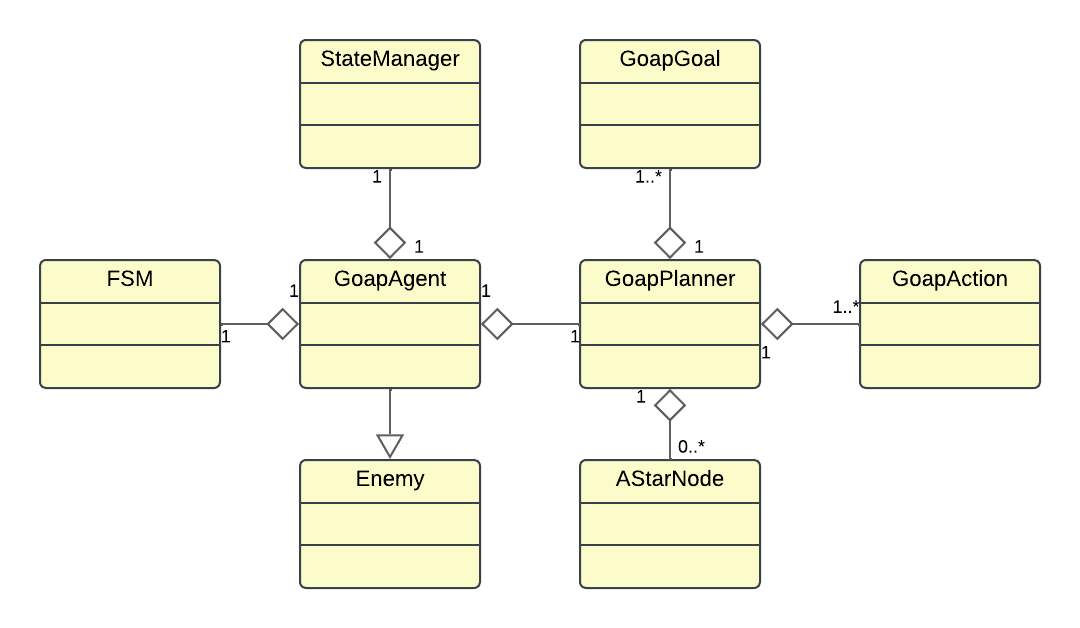
\includegraphics[width=16cm]{GOAP_2/GOAP_UML}
	\captionsetup{justification=justified, format=plain}
  \caption{GOAP Architektur}
  \label{GOAP Architektur eines Agenten}
\end{figure}

Aus dem GOAP-Kapitel geht hervor, dass ein GOAP-System aus einem Planner, Zielen, Aktionen und einer FSM (Finite State Machine) besteht. Diese Komponenten erfüllen ihre jeweiligen Aufgaben, wie im Grundlagenkapitel über GOAP beschrieben.

Der GoapAgent bildet dabei die Hauptklasse und soll die Schnittstelle zur restlichen Spielwelt sein. Die Spielwelt kann ihm Informationen wie die Position des Spielers oder bestimmte Koordinaten innerhalb der Spielwelt übermitteln. Dabei erbt der GoapAgent von der Klasse Enemy. Die Klasse Enemy stellt Komponenten bereit, die es dem GoapAgent ermöglichen, mit der Spielwelt zu interagieren.

Der StateManager verwaltet die Zustände des NPC. Diese Zustände können über die Komponenten der Oberklasse Enemy verändert werden können.

Die FSM setzt die Aktionssequenz aus, welche im GoapAgent gespeichert wird. Sie kann neue Sequenzen an den Goap gent anfordern.

Zur Generierung von Sequenzen und Festlegung des Zieles benutzt der GoapAgent die Klasse GoapPlanner. Der GoapPlanner besitzt dabei Objekte der Klasse GoapGoal. Aus diesen Objekten entscheidet sich der GoapPlanner für ein Zielzustand, zu welchem eine Aktionssequenz gesucht wird.
Der GoapPlanner sucht seine Sequenz mithilfe des A* Suchalgorithmus. Die Klasse AStarNode wird zur Erstellung von Knoten für den A* Suchalgorithmus benötigt. Ein AStarNode setzt dabei die Eigenschaften eines Suchbaum-Knoten um [siehe Kapitel Suchproblem, Knoten].

Die Klasse GoapAction definiert die Basisklasse für Aktionen. Eine Aktion repräsentiert dabei eine Kante im Suchbaum und wird entsprechend als solche im AStarNode-Objekt gespeichert.



\subsection{GoapAgent}

Folgende Abbildung stellt die Klasse GoapAgenten dar. Der GoapAgent speichert den GoapPlanner und die FiniteStateMachine als Objektvariable. Das action\_sequence Array speichert Klassenattribute des Typs GoapAction. Bei den Methoden handelt es sich \_process, get\_action\_sequence, und request\_plan. Die Darstellung wird anhand eines Klassendiagramms in UML-Notation umgesetzt.

\begin{figure}[h]
  \centering
  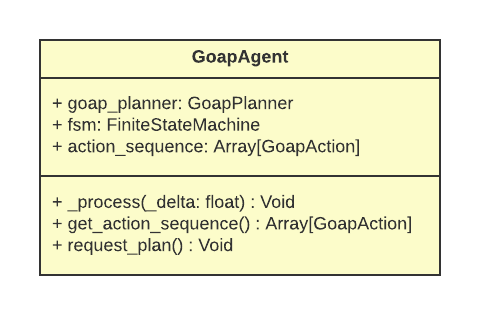
\includegraphics[width=10cm]{GOAP_2/GoapAgent_UML}
	\captionsetup{justification=justified, format=plain}
  \caption{GOAP Agent}
  \label{GOAP Agent}
\end{figure}

Die Methode \_process(delta: float) ist eine von Godot bereitgestellte Funktion, die jeden Frame aufgerufen wird, um kontinuierliche Logik wie Bewegungen, Animationen oder Eingaben zu verarbeiten. Mit hilfe dieser Methode werden Methoden anderer Klassen aufgerufen. Der Parameter delta repräsentiert die Zeit seit dem letzten Frame und könnte an andere Methoden übergeben werden.

\lstinputlisting[firstline=2, language=Godot, linerange={13,16-20}, caption={GoapAgent Klasse}, label=lst:caption]{code/goap_enemy.gd}

Die Getter-Methode get\_action\_sequence gibt das action\_sequence Array zurück, um es der aufrufenden Objektvariable FSM zur Verfügung zu stellen.

Die request\_plan Methode soll dem GoapAgent signalisieren, dass eine neue Sequenz an Aktionen benötigt wird, da diese zum jetzigen Zustand nicht gültig ist oder abgeschlossen wurde. Die Methode wird ebenfalls von der Objektvariable FSM aufgerufen. Somit würde der GoapAgent einen neue Seqeuenz an den GoapPlanner anfragen.

\subsection{GoapPlanner}

Folgende Abbildung zeigt die Struktur des GoapPlanner, anhand eines Klassendiagramms in UML-Notation. Die Klasse besteht aus den Arrays actions, goals und current\_plan, den Dictionaries effect\_action\_table und current\_state, sowie den Boolean create\_plan.

\begin{figure}[h]
  \centering
  \includegraphics[width=10cm]{GOAP_2/GoapPlanner_UML}
	\captionsetup{justification=justified, format=plain}
  \caption{GoapPlanner}
  \label{GoapPlanner}
\end{figure}

Die Methode update ist dabei die Methode, welche von der \_process Methode des GoapAgent aufgerufen wird. Von update werden weitere  Methoden und Abfragen durchgeführt. Einer der Methoden ist get\_best\_plan(), welche das Ziel aus dem goal Array auswählt. Wird eine neue Sequenz angefordert oder ändert sich das Ziel während der Laufzeit, so soll eine neue Sequenz gesucht werden. Die Suche geschieht über die Methode \textit{create\_new\_plan}.

\lstinputlisting[firstline=2, language=Godot, linerange={16-22}, caption={\textit{update} Methode des GoapAgent}, label=lst:caption]{code/goap_a_star_planner.gd}

Über \textit{create\_new\_plan} werden Zustände des Zieles nach dem derzeitigen Zustand des Agenten überschrieben. Dieser Zustand wird als Zustand des Wurzelknoten dienen, mit dem die a\_star\_algorithm Methode nach der Sequenz sucht. Die Funktionsweise der a\_star\_algorithm Methode wird in der folgenden Abbildung kommentiert.

\lstinputlisting[firstline=2, language=Godot, linerange={42-59}, caption={A* Algorithmus des GoapPlanner}, label=lst:caption]{code/goap_a_star_planner.gd}

Man beachte, dass Godot 4.3 keine PriorityQueue besitzt und man diese selbst umsetzen müsste. Eine PriorityQueue speichert Knoten sortiert nach ihren $f(n)$ Kosten, sodass Knoten mit den niedrigsten Kosten bevorzugt abgerufen werden. Die Umsetzung befindet sich im Anhang.

Die expand\_node Methode fügt Kindknoten des expandierten Knoten in die open\_list, welche vorher von A$^*$ gewählt wurde. Es folgt die Instanziierung der Kosten $g(n)$, $h(n)$ und $f(n)$ der Kindknoten und die Hinzufügung in die \textit{open\_list}.

\lstinputlisting[firstline=2, language=Godot, linerange={61-79}, caption={Expandierungs Methode des GoapPlanner}, label=lst:caption]{code/goap_a_star_planner.gd}

Die get\_child\_nodes Methode sucht nach Kanten (Aktionen) welche die benötigten Zustände des Knoten erfüllen können. Dabei werden die benötigten Zustände mit den Zuständen der effect\_action\_dict verglichen.

\begin{lstlisting}[language=dict, caption={effect\_action\_dict aus der Implementierung}]
effect_action_dict = {
    "player_eliminated": [
        RangedAttackFromCover:<Node#82829117475>,
        MeleeAttack:<Node#82845894692>,
        RangedAttack:<Node#82812340258>
    ],
    "player_block_visited": [
        GoToNode:<Node#82862671909>
    ],
    "at_patrol_node": [
        GoToNode:<Node#82862671909>
    ],
    "at_cover_node": [
        GoToNode:<Node#82862671909>
    ],
    "bullets": [
        Reload:<Node#82879449126>
    ]
}
\end{lstlisting}

Das Dictionary speichert alle Zustände als \textit{key} und die Aktionen, welche den Zustand beeinflussen können als \textit{values}. So erhält man eine schnellere Zugriffszeit, als wenn man jeden Effekt einer Aktion im Array mit dem benötigten Zustand vergleicht. 

Wird eine Aktion gefunden, welche den Zustand erfüllt, so wird untersucht ob der Effekt, der Aktion den Zustand umsetzen kann. Erfüllt der Effekt den gewünschten Zustand, so wird ein Kindknoten erstellt. Dieser Kindknoten speichert die Kante (Aktion) die zu dem Knoten geführt hat, sowie den Effekt auf den current\_state. Die restlichen Inhalte des Knoten werden in der zuvor beschriebenen expand\_node Methode instanziiert.

\lstinputlisting[firstline=2, language=Godot, linerange={90-107}, caption={Methode zur Suche nach möglichen Kanten}, label=lst:caption]{code/goap_a_star_planner.gd}

Wenn A$^*$ einen Knoten erweitert, der keine zu erfüllenden Zustände mehr besitzt, wurde der optimale Pfad gefunden. Um die korrekte Aktionssequenz zu erhalten, müssen die Aktionen der Knoten rekursiv vom Zielknoten bis zum Startknoten zurückverfolgt werden. Dies wird mithilfe der \textit{create\_path} Methode durchgeführt.



\subsection{AStarNode}

[...]

\begin{figure}[h]
  \centering
  \includegraphics[width=10cm]{GOAP_2/AStarNode_UML}
	\captionsetup{justification=justified, format=plain}
  \caption{AStarNode}
  \label{AStarNode}
\end{figure}

Der AStarNode geht nach einem Knoten eine Suchbaums [siehe Kapitel: Knoten eines Suchbaums]. Er speichert die bis dahin erfüllten Zustände im Attribut current\_state\_of\_goals, sowie alle Zielzustände die bis zu dem Knoten benötigt werden im Attribut goal\_state. Die Objektvariable parent_node speichert den Elternknoten, um später rekursiv auf die Kanten zurückschließen zu können. Die Kanten die zum Knoten geführt haben werden als GoapAction Objekt in der Objektvariable action gespeichert. 

Die Kosten $f(n)$ werden unter f\_cost und $g(n)$ -Kosten unter g\_cost gespeichert. Die Berechnung der Kosten passiert durch die GoapPlanner Methode expand\_node und werden über die setter- Methoden des AStarNode set\_g\_cost und set\_f\_cost initialisiert. Die Heuristik Kosten werden in der expand\_node Methode des GoapPlanner berechnet. Über die Methode get\_unsatasfied\_states werden alle Zustände zurückgegeben, welche noch nicht erreicht wurden. Die Größe des 




\subsection{GoapGoal}

Die Klasse \textit{GoapGoal} wird in der folgenden Abbildung mittels UML-Notation dargestellt. 

\begin{figure}[h]
  \centering
  \includegraphics[width=10cm]{GOAP_2/GoapGoal_UML}
	\captionsetup{justification=justified, format=plain}
  \caption{GoapGoal}
  \label{GoapGoal}
\end{figure}

Die Informationen zur Priorität und Gültigkeit werden aus der Objektvariable state\_manager gelesen. Die get\_best\_goal des GoapPlanner benötigt die Gültigkeit und Priorität, um in folge dessen das Ziel auszuwählen. Die Abfragen geschehen durch die Methoden get\_priority und is\_valid. Ein Ziel wird erst dann berücksichtigt, wenn es durch die Methode is\_valid als gültig bestätigt wurde. Anschließend kann dessen Priorität mithilfe von get\_priority ermittelt werden. 

Über die Methode get\_desired\_state werden die Zielzustände aufgerufen, welche der GoapPlanner zur Suche der Sequenz benötigt. 

Die Methode get\_goal\_name gibt den Namen des GoapGoals zurück, welche von Debug Methoden genutzt werden kann.



\subsection{GoapAction}

Abbildung [Nummer] stellt die GoapAction Klasse nach UML-Notation dar.

\begin{figure}[h]
  \centering
  \includegraphics[width=10cm]{GOAP_2/GoapAction_UML}
	\captionsetup{justification=justified, format=plain}
  \caption{GoapAction}
  \label{GoapAction}
\end{figure}

Mit hilfe der Objektvariablen character\_body und state\_manager werden die Kosten $g(n)$ und die Gültigkeit der Aktion gelesen. Die Kosten $g(n)$ werden dabei über die get\_cost Methode berechnet. Für die Rückgabe der Gültigkeit ist die is\_valid Methode zuständig. Die is\_valid Methode wird dabei für die Suche nach der Aktion genutzt, sowie während der Ausführung durch die FSM. Der GoapPlanner wählt nur Aktionen, welche im derzeitigen Zustand des NPC auch durchführbar sind. Auch die FSM prüft die Gültigkeit der Aktionen, da diese zu späterer Zeit ausgeführt werden können und sich der Zustand wieder ändern kann und somit auch die Gültigkeit.

Eine get\_preconditions Methode gibt die vorausgesetzten Zustände zurück, welche von anderen Aktionen erfüllt werden können. Ob eine Aktion einen Zustand erfüllen kann, hängt von der get\_effects Methode ab, welche ein \textit{Dictionary} mit dem Zustand und dessen Wert zurückgibt. Stimmt der Wert des Zustands mit dem Zielzustand überein, dann erfüllt die Aktion den Zustand.

Die update Methode leitet die eigentliche Ausführung der Aktion ein und wird von der FSM gestartet. Die Hoffnung dabei ist, dass die Aktion den erwünschten Wert des Effekts umsetzt. Aufgrund der nicht-deterministischen Natur der Spielwelt kann es jedoch vorkommen, dass der angestrebte Effekt nicht erreicht wird. Wird der Effekt nicht erreicht, so wird eine neue Sequenz angefordert oder das Ziel ändert sich bis dahin. Die Ausführung der Aktion wird dabei über Komponenten der Klasse Npc umgesetzt. Die Methode get\_action\_name gibt den Namen der Aktion zurück.

\lstinputlisting[firstline=2, language=Godot, linerange={}, caption={Die Aktion RangedAttack erbt von GoapAction}, label=lst:caption]{code/goap_ranged_attack.gd}

